\documentclass[a4paper]{article}
\usepackage[fontsize=13pt]{scrextend}
\usepackage[utf8]{vietnam}
\usepackage{amsmath}
\usepackage{amsfonts}
\usepackage{xcolor}
\usepackage{titlesec}
\usepackage{mdframed}
\usepackage{amssymb}
\usepackage{pgf,tikz,pgfplots}
\usepackage{graphicx}
\graphicspath{ {figures/} }
\usepackage{array}
\usepackage{cases}
\usepackage{listings}
\usepackage{tabulary}
\usepackage{color}
\usepackage{float} 
\usepackage{hyperref}
\usepackage{multirow}
\usepackage{minitoc}
\pgfplotsset{compat=1.5}
\usepackage{mathrsfs}
\usetikzlibrary{arrows, calc}
\usepackage{fancyhdr}
\usepackage{longtable}
\usepackage{verbatim}
\usepackage{indentfirst}
\pagestyle{fancy}
\pagestyle{empty}
\definecolor{dkgreen}{rgb}{0,0.6,0}
\definecolor{gray}{rgb}{0.5,0.5,0.5}
\definecolor{mauve}{rgb}{0.58,0,0.82}
\lstset{frame=tb,
  language=C++,
  aboveskip=3mm,
  belowskip=3mm,
  showstringspaces=false,
  columns=flexible,
  basicstyle={\small\ttfamily},
  numbers=none,
  numberstyle=\tiny\color{gray},
  keywordstyle=\color{blue},
  commentstyle=\color{dkgreen},
  stringstyle=\color{mauve},
  breaklines=true,
  breakatwhitespace=true,
  tabsize=3
}
\hypersetup{
    colorlinks=true,
    linkcolor=black,
    filecolor=magenta,      
    urlcolor=red,
    pdftitle={Báo cáo đồ án Remote Desktop},
	% pdfpagemode=FullScreen,
    }
\renewcommand{\listfigurename}{Danh sách hình}
\renewcommand{\listtablename}{Tables}
\newcommand{\tabitem}{~~\llap{\textbullet}~~}
\usepackage[left=2cm,right=2cm,top=2cm,bottom=2cm]{geometry}
\author{Tạ Chí Thành Danh}
\newmdenv[linecolor=black,skipabove=\topsep,skipbelow=\topsep,
leftmargin=-5pt,rightmargin=-5pt,
innerleftmargin=5pt,innerrightmargin=5pt]{mybox}
\fancyhf{}
\lhead{Báo cáo đồ án Mạng máy tính}
\chead{}
\rhead{}
\cfoot{\thepage}
\rfoot{}
\lfoot{}
\pagestyle{fancy}
\renewcommand{\headrulewidth}{0pt}
\renewcommand{\footrulewidth}{0pt}
\begin{document}
\begin{titlepage}
\begin{mybox}
\begin{center}
\fontsize{12}{12}\selectfont
\textbf{ĐẠI HỌC QUỐC GIA THÀNH PHỐ HỒ CHÍ MINH}\\
\textbf{TRƯỜNG ĐẠI HỌC KHOA HỌC TỰ NHIÊN}\\
\textbf{KHOA CÔNG NGHỆ THÔNG TIN}
\end{center}
\vskip 1 cm
\begin{figure}[H]
\begin{center}

\includegraphics[scale=0.25]{figures/logo}
\end{center}
\end{figure}
\vskip 1 cm
\begin{center}
\fontsize{18}{14}\selectfont
\textbf{BÁO CÁO ĐỒ ÁN MÔN HỌC}\\
\fontsize{26}{16}\selectfont
\textbf{MẠNG MÁY TÍNH}\\
\fontsize{18}{12}\selectfont
\textbf{ĐỀ TÀI: Điều khiển máy tính thông qua ứng dụng Desktop}
\end{center}
\vskip 1 cm
\fontsize{14}{12}\selectfont
\textbf{Giảng viên lý thuyết:} Thầy Đỗ Hoàng Cường\\
\textbf{Giảng viên thực hành:} Cô Huỳnh Thuỵ Bảo Trân\\
\textbf{Lớp:} 22TNT1TN\\
\textbf{Thành viên thực hiện:}
\begin{itemize}
\item 22120025 $-$ Nguyễn Long Bảo
\item 22120044 $-$ Nguyễn Cao Cường
\item 22120049 $-$ Tạ Chí Thành Danh
\end{itemize}
\vskip 3 cm
\begin{center}
\textbf{THÀNH PHỐ HỒ CHÍ MINH, THÁNG 12 NĂM 2023}
\end{center}
\end{mybox}
\end{titlepage}

\tableofcontents
\listoffigures
\listoftables
\newpage

\section{Giới thiệu}
\subsection{Tổng quan}
Ứng dụng cho phép một quản trị viên hoặc người dùng (sử dụng ứng dụng với vai trò là \textbf{Admin} hay máy Client) điều khiển một máy tính từ xa (máy Server) trong cùng mạng LAN với máy Server. Ứng dụng sử dụng \textbf{socket}, giao thức \textbf{TCP} ở tầng Transport, và được lập trình bằng ngôn ngữ C++. Dưới đây là các chức năng của ứng dụng:
\begin{itemize}
	\item Kết nối đến máy Server qua địa chỉ IP: Cho phép thiết lập kết nối tới máy chủ thông qua việc nhập địa chỉ IP.
	\item Đăng nhập với vai trò admin hoặc user bình thường: Cung cấp tính năng đăng nhập với vai trò quản trị hoặc người dùng thông thường, đảm bảo quyền truy cập phù hợp.	
	\item Ngắt kết nối với một địa chỉ IP: Cho phép ngắt kết nối tới máy tính có địa chỉ IP cụ thể trong cùng mạng LAN.
	\item Chia sẻ màn hình hiện tại: Hiển thị và chia sẻ màn hình hiện tại của máy tính Server.
	\item Gửi tín hiệu chuột đến máy bị điều khiển: Điều khiển các thao tác chuột từ xa đến máy tính được điều khiển.
	\item Gửi tín hiệu bàn phím đến máy bị điều khiển: Cho phép điều khiển bàn phím từ xa trừ các tổ hợp phím đặc biệt như Ctrl + Alt + Del.
\end{itemize}

\subsection{Về Socket}
Socket là là một giao diện lập trình ứng dụng (API) cho việc giao tiếp mạng giữa các ứng dụng mạng. Socket cung cấp cơ chế gửi và nhận dữ liệu, thiết lập kết nối và quản lý các thông tin liên quan đến mạng như địa chỉ IP và Port number.

Ứng dụng sử dụng socket hướng kết nối: dựa trên giao thức TCP, việc truyền dữ liệu
chỉ thực hiện giữa 2 quá trình đã thiết lập kết nối. Giao thức này đảm bảo dữ liệu được
truyền đến nơi nhận một cách đáng tin cậy, đúng thứ tự nhờ vào cơ chế quản lý luồng
lưu thông trên mạng và cơ chế chống tắc nghẽn. Đồng thời, mỗi thông điệp gửi phải có
xác nhận trả về và các gói tin chuyển đi tuần tự.
\subsection{Công cụ}
\subsubsection{wxWidgets}
wxWidgets là một thư viện mạnh mẽ và linh hoạt cho phát triển giao diện người dùng đa nền tảng bằng ngôn ngữ lập trình C++. Trong đồ án này, wxWidgets được sử dụng để thiết kế giao diện cho ứng dụng, đồng thời hỗ trợ việc xử lí các sự kiện từ phía Client và Server trong quá trình gửi và nhận các thông tin qua socket.

Thư viện này cung cấp các thành phần giao diện đồ hoạ như cửa sổ, nút bấm, hộp thoại và menu, giúp tạo ra giao diện người dùng trực quan và dễ sử dụng. Đặc biệt, wxWidgets cho phép triển khai ứng dụng trên nhiều hệ điều hành khác nhau một cách dễ dàng mà không cần phải viết lại mã nguồn.

Việc sử dụng wxWidgets giúp nhóm tập trung vào việc thiết kế giao diện và chức năng điều khiển từ xa mà không cần quá lo lắng về sự không tương thích giữa các nền tảng hệ điều hành. Thư viện cũng cung cấp tài liệu phong phú và có cộng đồng hỗ trợ đông đảo, giúp việc học và phát triển ứng dụng trở nên dễ dàng hơn.
\subsubsection{Asio}

Thư viện Asio là một thư viện mã nguồn mở mạnh mẽ cho ngôn ngữ lập trình C++, được sử dụng để thực hiện việc lập trình mạng và giao tiếp qua mạng một cách linh hoạt và hiệu quả.

Asio cung cấp các công cụ và lớp trừu tượng để tạo, quản lý và tương tác với các kết nối mạng, bao gồm cả việc xử lý socket, thiết lập kết nối, gửi và nhận dữ liệu trên mạng. Đặc biệt, nó hỗ trợ cả các giao thức đồng bộ (ví dụ như TCP) và không đồng bộ (ví dụ như UDP), cho phép việc truyền dữ liệu một cách đáng tin cậy và nhanh chóng.

Asio được thiết kế để linh hoạt và dễ sử dụng, với cách tiếp cận dựa trên bất đồng bộ (asynchronous), cho phép thực hiện các hoạt động mạng mà không cần chờ đợi kết quả trả về từ mỗi yêu cầu riêng biệt. Điều này làm cho việc xây dựng ứng dụng mạng với hiệu suất cao trở nên dễ dàng hơn, đặc biệt trong việc xử lý hàng loạt yêu cầu từ nhiều nguồn khác nhau.

Trong đồ án này, nhóm tập trung sử dụng chủ yếu với chức năng thiết lập kết nối TCP của nó. Sự linh hoạt và hiệu suất của Asio trong việc xử lý giao tiếp mạng bất đồng bộ đã hỗ trợ nhóm trong việc xây dựng và quản lý việc truyền dữ liệu đáng tin cậy giữa các thiết bị qua mạng.
\subsubsection{Windows API}
Windows API (Application Programming Interface) là bộ công cụ mạnh mẽ của hệ điều hành Windows, cung cấp chức năng và dịch vụ cần thiết cho việc tương tác ứng dụng Windows với hệ thống và phần cứng.

Trong quá trình phát triển ứng dụng Remote Desktop Control, nhóm đã tận dụng tính linh hoạt của Windows API để thực hiện các thao tác điều khiển từ xa. Chúng tôi đã sử dụng Windows API để gửi các yêu cầu tương ứng với các thao tác như nhấn phím, di chuyển con chuột, và thực hiện các thao tác click chuột trên máy tính được điều khiển.

Hơn nữa, thông qua Windows API, chúng tôi đã có thể truy xuất và lấy thông tin cơ bản của máy tính được kết nối, như địa chỉ IP và địa chỉ MAC, giúp quản lý và xác định máy tính từ xa một cách chính xác.

Bằng cách tích hợp các tính năng linh hoạt của Windows API vào ứng dụng Remote Desktop Control, chúng tôi đã tạo ra một trải nghiệm điều khiển từ xa hiệu quả và ổn định, mang lại sự linh hoạt và tiện ích cho người dùng.
\newpage
\section{Các chức năng của phần mềm}
\subsection{Giao diện của ứng dụng khi khởi động}
Khi mở ứng dụng, giao diện ban đầu của ứng dụng là màn hình đăng nhập, ở đây ta có thể đăng nhập với 2 vai trò đó là User bình thường (Server) hoặc Admin (Client). Mặc định thì ứng dụng sẽ hiển thị ô đăng nhập với vai trò là User, để đăng nhập với vai trò Admin thì ta tích vào ô ``\textbf{Login as ADMIN}``. (Hình \ref{fig:ServerLogin} và Hình \ref{fig:ClientLogin})

\begin{figure}[H]
	\centering{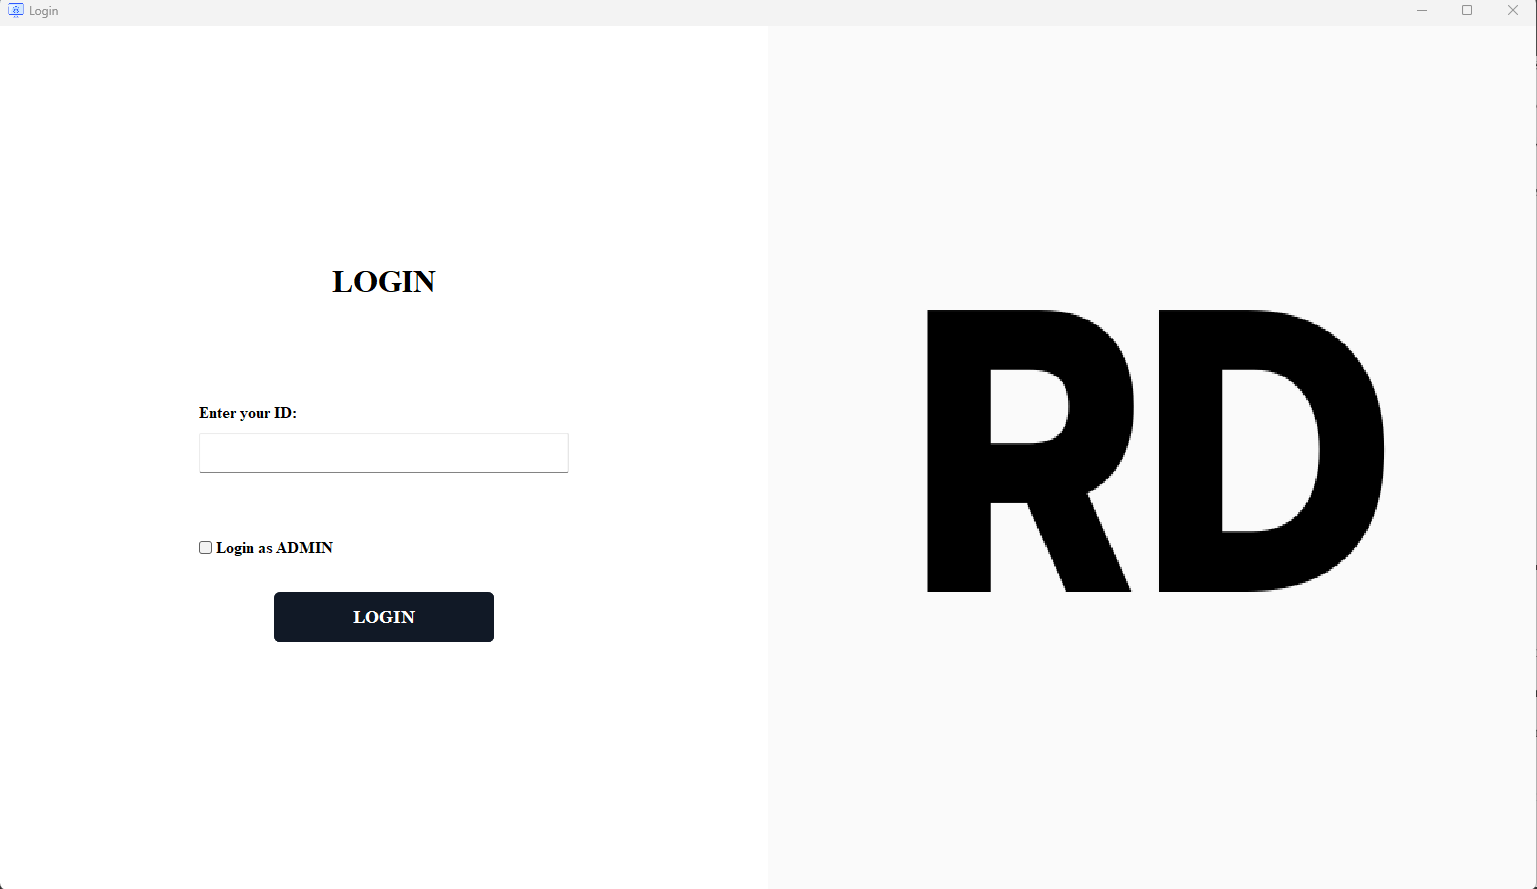
\includegraphics[scale=0.35]{ServerLoginWindow}}
	\caption{Màn hình đăng nhập của User}
	\label{fig:ServerLogin}
\end{figure}

\begin{figure}[H]
	\centering{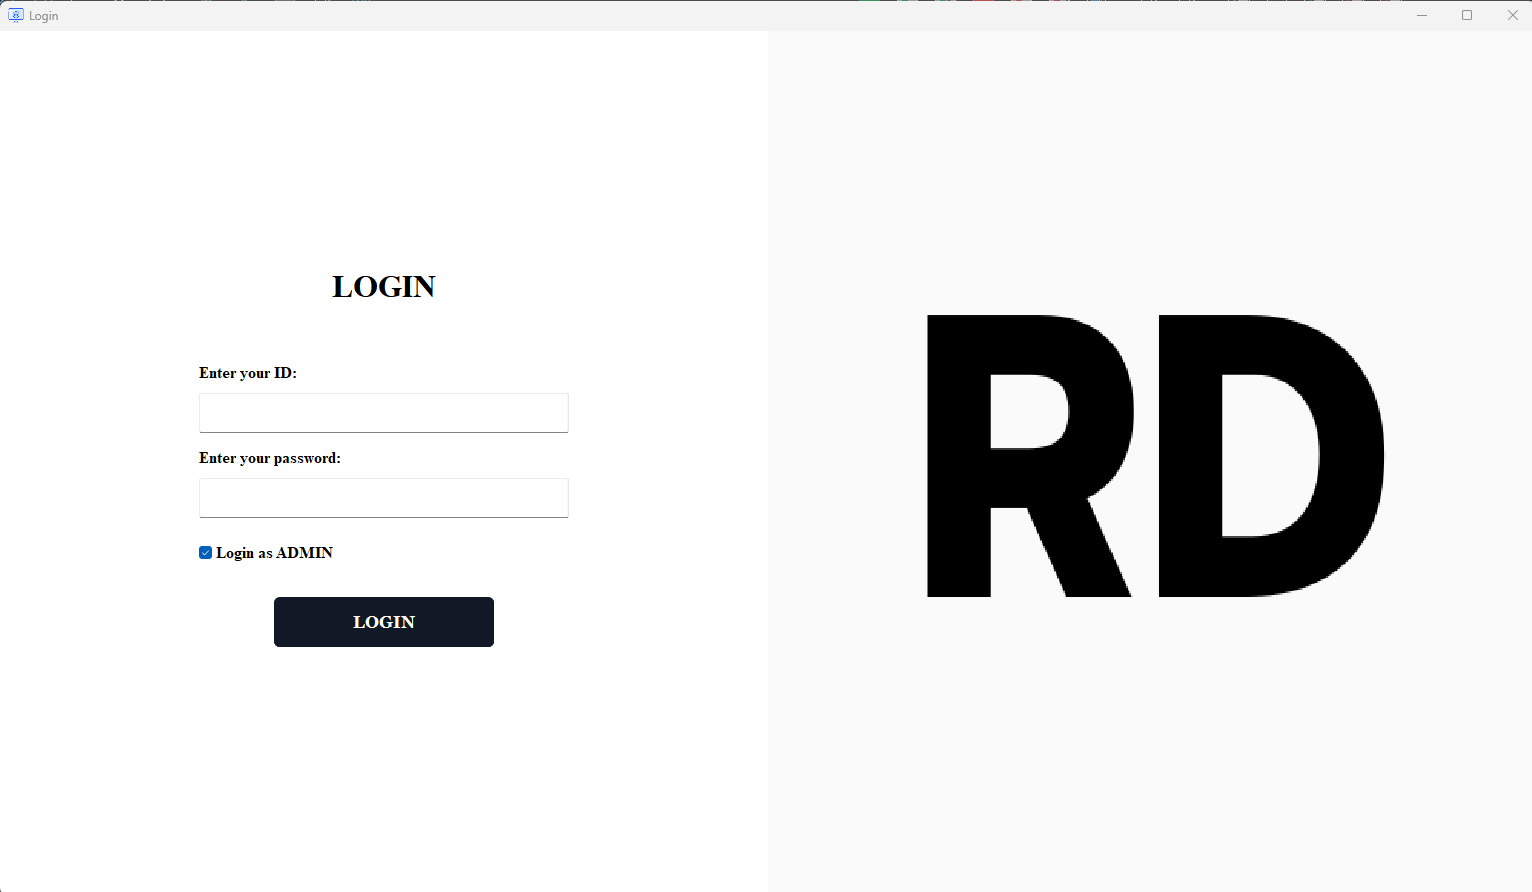
\includegraphics[scale=0.35]{ClientLoginWindow}}
	\caption{Màn hình đăng nhập của Admin}
	\label{fig:ClientLogin}
\end{figure}

Để đăng nhập được với vai trò là User, ta cần nhập tên đăng nhập là một chuỗi ký tự ASCII với độ dài từ 4 đến 10 ký tự. Còn đối với Admin thì tên đăng nhập và mật khẩu mặc định là \verb|admin|.
\subsection{Giao diện của ứng dụng sau khi đăng nhập}
\subsubsection{Giới thiệu}
Sau khi đăng nhập xong, ứng dụng chuyển sang giao diện chính, đây là nơi người dùng sử dụng các chức năng chính của ứng dụng. Màn hình chính sau khi đăng nhập xong như sau:
\begin{figure}[H]
	\centering{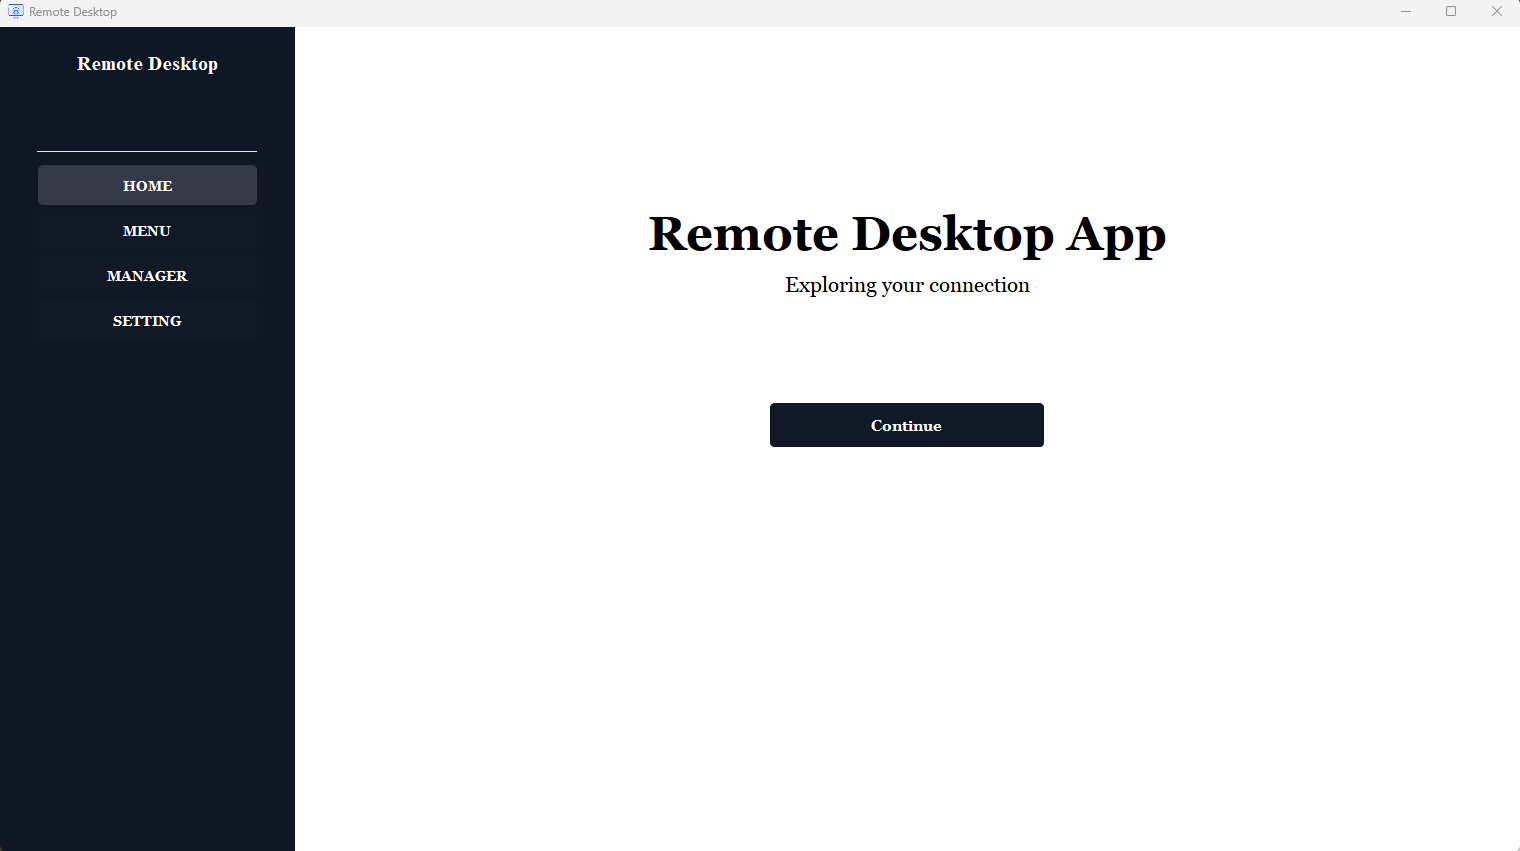
\includegraphics[scale=0.4]{MainWindow}}
	\caption{Màn hình chính của ứng dụng}
	\label{fig:ServerLogin}
\end{figure}
Ở thanh điều hướng, ta có 4 nút chức năng đó là nút \textbf{Home}, \textbf{Menu}, \textbf{Manager}, \textbf{Setting}. Nội dung của màn hình \textbf{Home} là màn hình chính sau khi đăng nhập vừa trình bày ở trên, còn giao diện của các màn hình tương ứng với các nút sẽ được mô tả ở những mục tiếp theo.

Khi người dùng ấn nút Menu trên cửa sổ chính của ứng dụng, ở khu vực hiển thị bên phải sẽ thay đổi tuỳ theo việc người dùng đang đăng nhập với vai trò là \textbf{Admin} (tức \textbf{Client}) hay \textbf{User thông thường} (tức \textbf{Server}).

\subsection{Màn hình Menu của Client}
\subsubsection{Mô tả}
Dưới đây là nội dung hiển thị tương ứng với vai trò \textbf{Admin} (\textbf{Client}):
\begin{figure}[H]
	\centering{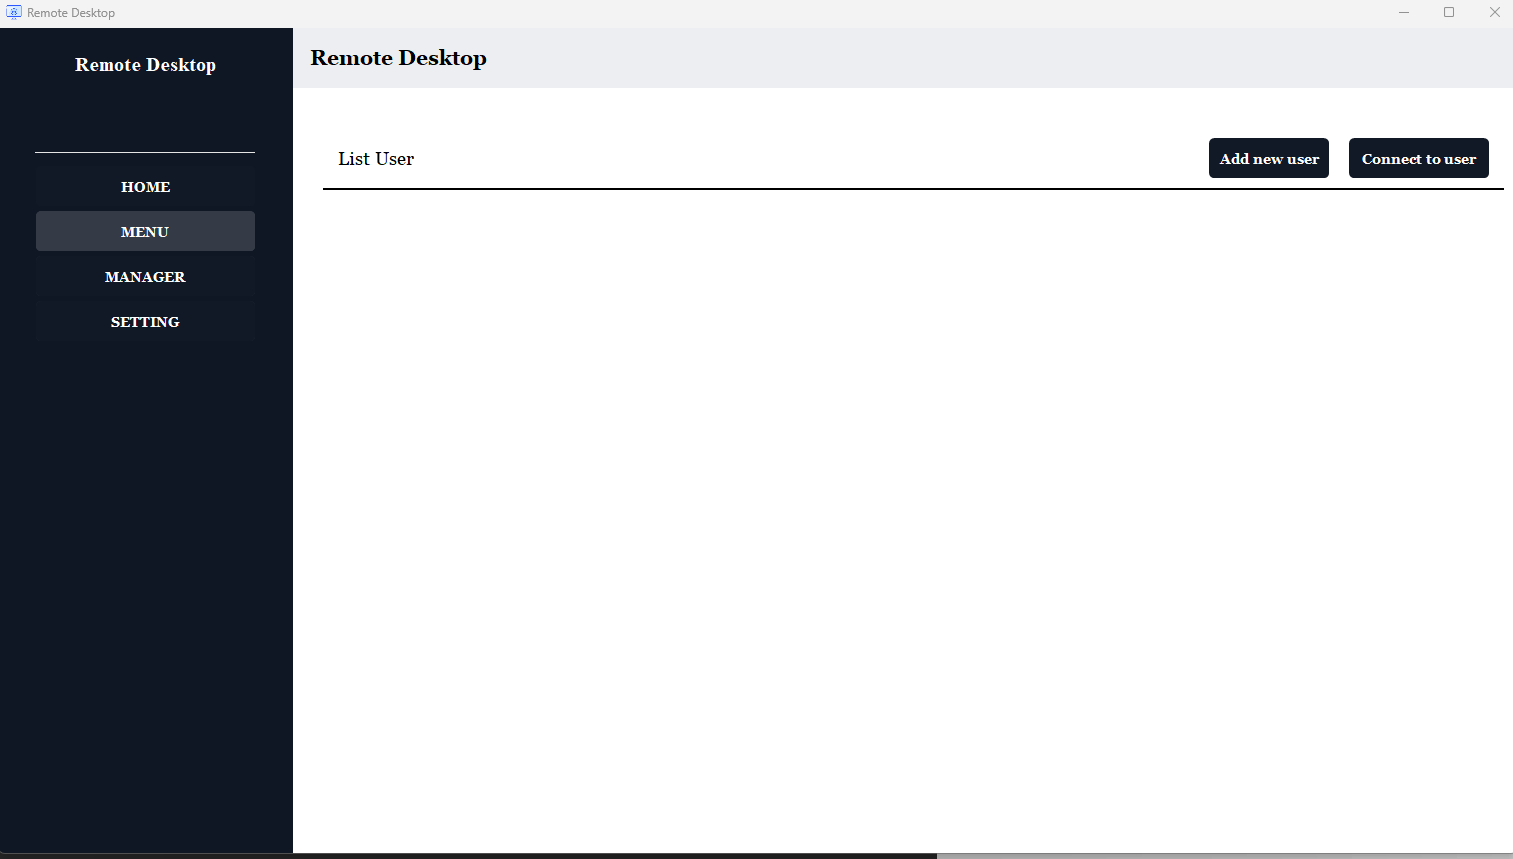
\includegraphics[scale=0.4]{ClientMenuWindow}}
	\caption{Màn hình chính của ứng dụng}
	\label{fig:ClientMenuWindow}
\end{figure}
Ở màn hình menu của 
\subsubsection{Hướng dẫn sử dụng}

\subsection{Màn hình Manager}
Màn hình Manager phục vụ những chức năng sau:
\begin{itemize}
	\item Quản lý Người Dùng: Màn hình Manager thường cung cấp chức năng quản lý người dùng, cho phép tạo và xóa người dùng ra khỏi danh sách kết nối, cũng như cấp quyền truy cập tương ứng.	
	\item Xác Thực và Quản Lý Quyền Truy Cập: Màn hình Manager thường cung cấp cơ chế xác thực để đảm bảo chỉ người dùng được ủy quyền mới có thể thực hiện các thao tác quản lý như ngắt kết nối, điều khiển từ xa và quản lý người dùng.	
	\item Ghi Log và Theo Dõi Hoạt Động: Có thể có chức năng ghi log hoạt động của người dùng, bao gồm việc kết nối, thao tác từ xa và các hoạt động khác. Điều này giúp theo dõi và đánh giá hoạt động trên hệ thống.	
\end{itemize}
Màn hình Manager là trung tâm quản lý chính, cung cấp khả năng kiểm soát và quản lý toàn diện về người dùng và kết nối từ xa. Việc có một công cụ quản lý mạnh mẽ như vậy giúp cải thiện hiệu suất và an ninh trong việc sử dụng và quản lý các kết nối từ xa. Đây là tính năng đang được nhóm dự định phát triển và mở rộng trong tương lai.











\subsection{Cửa sổ Setting}
Cửa sổ Settings (Cài đặt) trong ứng dụng Remote Desktop Control thường là nơi người dùng có thể tinh chỉnh và điều chỉnh các cài đặt và tuỳ chọn cho ứng dụng. Các tính năng và chức năng chính của cửa sổ Settings bao gồm:
\begin{itemize}
	\item Cài đặt Kết Nối: Cho phép người dùng nhập địa chỉ IP hoặc tên máy chủ để thiết lập kết nối đến máy tính từ xa. Điều này có thể bao gồm cả cài đặt cổng kết nối và các thiết lập bảo mật.
	
	\item Tùy Chọn Giao Diện: Cho phép người dùng điều chỉnh giao diện của ứng dụng, bao gồm cỡ chữ, màu sắc, chủ đề, và các tuỳ chọn hiển thị khác để tương thích với sở thích và nhu cầu cá nhân.
	
	\item Quản lý Người Dùng: Cung cấp khả năng quản lý tài khoản người dùng, bao gồm việc thay đổi mật khẩu, cập nhật thông tin cá nhân và quyền truy cập.
	
	\item Cài Đặt Bảo Mật: Cho phép người dùng cấu hình các tùy chọn bảo mật như cấp quyền truy cập, xác thực, mã hóa dữ liệu để đảm bảo an toàn khi truy cập và điều khiển từ xa.
	
	\item Tùy Chọn Khác: Có thể bao gồm các tùy chọn khác như ngôn ngữ, cấu hình kết nối mạng, cài đặt proxy và các tùy chọn nâng cao khác.	
\end{itemize}
Cửa sổ Settings là nơi tập trung các tuỳ chọn và cài đặt quan trọng, cho phép người dùng cá nhân hóa và điều chỉnh ứng dụng theo nhu cầu và yêu cầu cụ thể của họ. Điều này giúp tăng cường trải nghiệm người dùng và cung cấp sự linh hoạt trong việc sử dụng ứng dụng Remote Desktop Control. Đây cũng là tính năng sẽ được nhóm phát triển sau.







\section{Tổ chức thư mục của chương trình}
Chương trình được tổ chức như sau.
Ở server:
\begin{figure}[H]
\centering{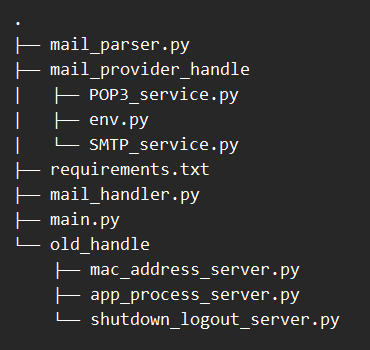
\includegraphics[scale=1]{server_dir}}
\caption{Tổ chức thư mục ở server}
\end{figure}
Server có thư mục \textbf{mail$\mathbf{\_}$provider$\mathbf{\_}$handle} chứa các module phục vụ cho quá trình gửi và nhận mail, thư mục \textbf{old$\mathbf{\_}$handle} chứa một vài hàm được cung cấp sẵn cho quá trình xử lý các yêu cầu. \\
Module \textbf{mail$\mathbf{\_}$parser.py} chứa hàm phục vụ cho quá trình phân tích lệnh được nhận từ email. Module \textbf{mail$\mathbf{\_}$handler} chứa các hàm xử lý yêu cầu, giao tiếp với client và trả kết quả. \\
Tập tin \textbf{requirements.txt} chứa các yêu cầu cần thiết (bên cạnh Python 3.9 trở lên) để chạy chương trình.\\
Tập tin \textbf{main.py} là tập tin chính của server, ta cần chạy tập tin này để khởi động server. \textbf{Lưu ý} khi chạy tập tin này, ta cần thay đổi giá trị \textbf{MAX$\mathbf{\_}$CONNECTION} ở dòng 13 thành giá trị \textbf{bằng đúng} với số lượng client (tối đa 4).
Ở client:
\begin{figure}[H]
\centering{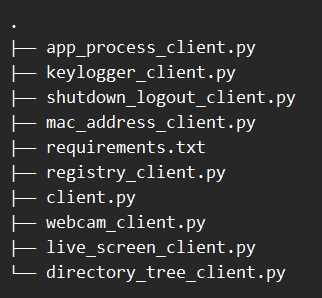
\includegraphics[scale=1]{victim_dir}}
\caption{Tổ chức thư mục ở client}
\end{figure}
Tập tin \textbf{requirements.txt} chứa các yêu cầu cần thiết (bên cạnh Python 3.9 trở lên) để chạy chương trình.\\
Trừ tập tin \textbf{client.py}, các tập tin mã nguồn Python còn lại chứa các hàm xử lý các yêu cầu được gửi đến từ server.\\
Tập tin \textbf{client} là tập tin chính của client, ta cần chạy tập tin này để khởi động client. \textbf{Lưu ý} khi chạy tập tin này ta cần thay đổi giá trị 127.0.0.1 ở dòng 60 thành một giá trị thích hợp.\\
\textbf{Tất cả các client phải được kết nối đến server TRƯỚC khi server bắt đầu nhận và xử lý các lệnh từ email.}


\section{Cú pháp email}
Các email điều khiển được gửi về địa chỉ \textbf{notabotbytheway@outlook.com}.\\ 
Các lệnh phải được viết ở \textbf{tiêu đề} của email.\\
Giá trị key là \textbf{1234}.\\
Cú pháp của các lệnh điều khiển được liệt kê bên dưới:
\begin{itemize}
\item \textbf{AUTH} <key> <IP>: "đăng ký" địa chỉ email để điều khiển <IP>. Tại một thời điểm, mỗi địa chỉ email đăng ký \textbf{duy nhất} với một địa chỉ IP và ngược lại.
\item \textbf{LIST} <key>: liệt kê danh sách các IP đang kết nối.
\item \textbf{DISC}: ngắt kết nối địa chỉ email này với IP hiện tại.
\item \textbf{LIST}$\_$\textbf{PROC}: liệt kê danh sách các tiến trình (process).
\item \textbf{LIST}$\_$\textbf{APP}: liệt kê danh sách các ứng dụng (application).
\item \textbf{KILL} <ID/PID>: tắt (kill) tiến trình có mã là <ID/PID>.
\item \textbf{SCREENSHOT} <time>: chụp màn hình liên tục trong thời gian <time> giây, mặc định là $0.5$ giây.
\item \textbf{WEB}/\textbf{REC} <time>: quay lại webcam của máy trong thời gian <time> giây, mặc định là $5$ giây. 
\item \textbf{KEYLOG} <time>: bắt các phím nhấn trong thời gian <time> giây, mặc định là $10$ giây.
\item \textbf{SHUTDOWN}: tắt máy tính.
\item \textbf{LOGOUT}: đăng xuất. % khỏi Trái Đất
\item \textbf{RESTART}: khởi động lại máy tính.
% \item \textbf{MAC}: lấy địa chỉ MAC.
\item \textbf{REGISTRY} \textbf{LIST} <path>: danh sách các registry trong path.
\item \textbf{REGISTRY} \textbf{UPDATE} <registry path> <value> <data type>: cập nhật giá trị của <registry path> thành <value> với kiểu <data type>. <value> \textbf{không} được có khoảng trắng. <data type> được lấy từ \href{https://docs.microsoft.com/en-us/windows/win32/sysinfo/registry-value-types}{link}.
\item \textbf{DIR} \textbf{LIST} <path>: liệt kê các thư mục/file trong đường dẫn <path>.
\item \textbf{DIR} \textbf{COPY} <source file> <destination path>: copy file có tên <source file> đến đường dẫn <destination path>.
\end{itemize}
\section{Kiến trúc ứng dụng: }
Tại phần này, chúng tôi sẽ trình bày về các thành phần chính của ứng dụng, mô tả cách mà các thành phần trong ứng dụng như Network, View, Model... có thể giao tiếp với nhau và các giao thức được định nghĩa trong phần Network.

\subsection{Kiến trúc Network: }
\label{sec:network-archi}
Ở phần này chúng tôi sẽ giới thiệu các thành phần cơ bản của Network. \\

\begin{figure}[H]
	\centering
	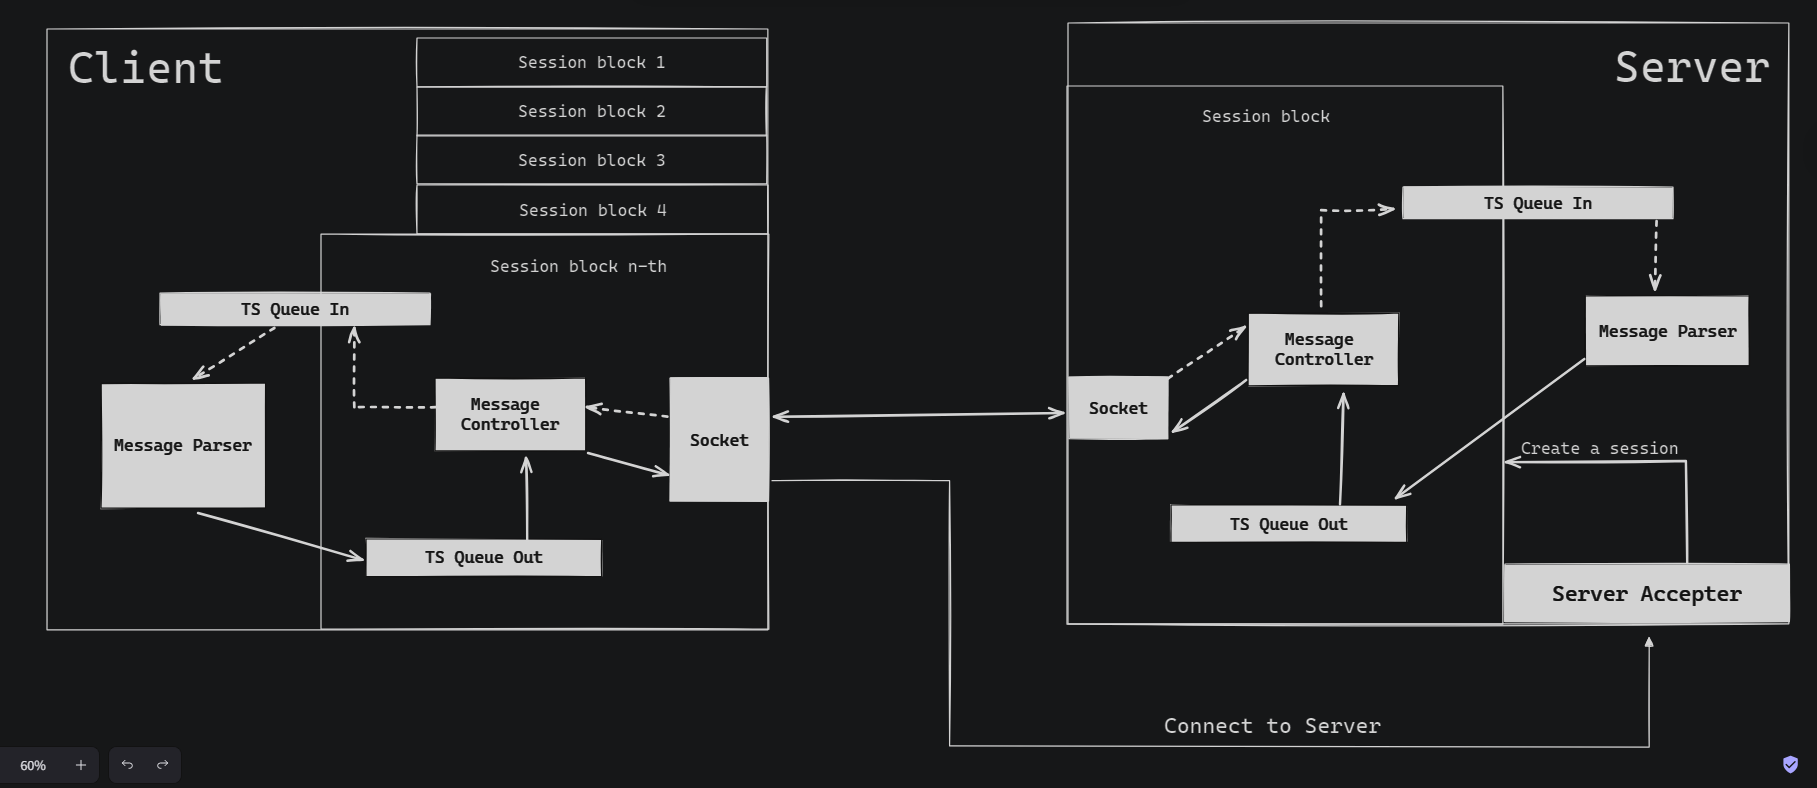
\includegraphics[width=\linewidth]{latex/architechture/architechture_diagram.png}
	\caption{Networking Architechture Diagram}
	\label{fig:network}
\end{figure}

Trên đây là mô hình cơ bản của kiến trúc network của chúng tôi và luồng di chuyển của message. Lưu ý: ở đây với mũi tên vẽ liền đại diện cho luồng di chuyển message \textit{ra ngoài}, còn mũi tên nét đứt đại diện cho message được gởi \textit{vào}.

\subsubsection{Message: }
\label{sec:message}
\textbf{Message} là dữ liệu cơ bản được truyền đi nhằm thực hiện giao tiếp giữa hai ứng dụng với nhau.

Kiểu dữ liệu được thiết kế gồm hai phần
\begin{itemize}
	\item \textbf{Header} chứa những thông tin cơ bản của message, ở đây là \underline{kích cỡ message} và \underline{loại message}, chi tiết về \underline{các loại message} sẽ được trình bày tại phần \textbf{Kiến Trúc Protocol}
	\item \textbf{Body} chứa \underline{toàn bộ dữ liệu của message}
\end{itemize}

Việc thiết kế thêm phần Header sẽ giúp cho việc giao tiếp giữa hai ứng dụng trở nên dễ dàng phân loại và quản lý hơn.

\subsection{ThreadSafe Queue: }

Là một kiểu dữ liệu quan trọng trong cấu trúc ứng dụng, được thiết kế để giải quyết tính tuần tự của các sự kiện, kết nối, message....  đảm bảo an toàn khi truy cập dữ liệu, không xảy ra mâu thuẫn, thiếu sót và tối ưu hóa việc sử dụng tài nguyên trong quá trình xử lý đa luồng của máy tính.

Kiểu dữ liệu này bản chất là một hàng đợi hai đầu, nhưng được tích hợp thêm khoá \textit{(Mutex)} và cơ chế \textit{Wait}, cụ thể như sau :
\begin{itemize}
	\item \textbf{Mutex} : Ở mỗi thao tác có sự tác động tới dữ liệu trong \textit{Queue}, chúng đều sẽ khoá \textit{Mutex} chung lại, đảm bảo rằng chỉ sau khi xử lý xong công việc mới được tiếp tục đi tới thao tác tác động tới dữ liệu khác, điều này đảm bảo tính nhất quán của dữ liệu trong \textit{Queue}, tránh mâu thuẫn và xung đột khi nhiều luồng cùng truy cập. Điều này rất quan trọng để đảm bảo an toàn khi xử lý đa luồng.
	\item \textbf{Cơ chế Wait} : nhằm tiết kiệm tài nguyên của máy tính, \textit{Queue} sẽ được đưa vào trạng thái chờ đợi \textit{(không sử dụng tài nguyên)} nếu nó rỗng, và chỉ trở lại hoạt động khi một phần tử mới được thêm vào.
\end{itemize}

\underline{Lưu ý}: ThreadSafe Queue được sử dụng cho mọi hàng đợi được tạo ra trong phần Network, vì thế để thuận tiện, kể từ bây giờ chúng tôi sẽ gọi là \textit{Hàng đợi} (\textit{Queue}) và ngầm hiểu đó là đối tượng \textit{ThreadSafe Queue}.

\subsubsection{Session: }
\textbf{Session} là thành phần chính của kiến trúc mạng của chúng tôi. Thành phần này được thiết kế như là nơi thực hiện việc giao tiếp trực tiếp với đối tượng bên ngoài thông qua socket. Mỗi session sẽ chỉ tạo với mỗi kết nối được thiết lập giữa \textit{Client} và \textit{Server} và được dùng để giao tiếp giữa chính hai đối tượng đó. Điều này giúp việc quãn lý bộ nhớ và các trạng thái một cách dễ dàng và tự động, giảm độ phức tạp trong việc xử lý gởi nhận trong quá trình giao tiếp.

Session chứa các đối tượng chính như là: 
\begin{itemize}
	\item \textbf{Socket} - Endpoint cho kết nối. Trong kiến trúc mạng của chúng tôi, chỉ session mới chứa socket để thực hiện giao tiếp.
	\item \textbf{IncommingQueue} - Hàng đợi message cho dữ liệu được nhận vào, được thiết kế là một đối tượng std::shared\_ptr và được tham chiếu bởi cả \textit{Session} và đối tượng chứa nó (\textit{Client} hoặc \textit{Server}). Khi \textit{Session} nhận được message từ bên ngoài, đối tượng này sẽ kiểm tra tính hợp lệ của message (theo phong cách đã được định nghĩa), sau đó sẽ được đưa vào xử lý bởi \textit{Client} và \textit{server}. Điều này giúp làm tránh các xung đột và những bất cập trong việc quãn lý khi một server có thể xử lý nhiều \textit{Session}. Khi đó, các đối tượng như \textit{Server} hay \textit{Client} có thể dễ dàng xử lý trong một hàng đợi duy nhất và gởi đi message mới cho đúng \textit{Session}.
	\item \textbf{OutcommingQueue} - Hàng đợi message cho dữ liệu gởi đi. Khác với \textit{IncommingQueue}, \textit{OutcommingQueue} chỉ được tham chiếu bởi \textit{Session}. Trong khi kết nối được thiết lập, \textit{Session} sẽ luôn kiểm tra \textit{OutcommingQueue} còn dữ liệu không, nếu có sẽ gởi tất cả những dữ liệu bên trong và đợi cho đến khi có message mới được thêm vào.
\end{itemize}

\subsubsection{IClient và IServer: }
\textit{IClient} và \textit{IServer} là hai abstract class tạo ra để quãn lý, phân phối và xử lý các event và message.  \\
Trong \textit{IClient} và \textit{IServer} đều được thiết kế các hàm để kết nối, chấp nhận kết nối, gởi và nhận các message từ \textit{Session} và quãn lý các \textit{Session} này. \textit{Client} và \textit{Server} chứa một hàng đợi gọi là \textit{IncommingQueue} như hình trên đã thể hiện. Chúng có nhiệm vụ nhận các message từ \textit{Session} và phân phối và xử lý dựa trên HeadID của message mà phân phối cho các handler phù hợp. \\
Trong cách implementation của mình, chúng tôi chỉ cho các class này tạo ra 2 \textit{Session} mỗi kết nối, một cho việc truyền dữ liệu ảnh từ \textit{Server} sang \textit{Client}, một dành cho việc truyền các event điều khiển từ \textit{Client} sang \textit{Server}. Việc này giúp dữ liệu ở \textit{Session} không bị tràn khi mà kích thước dữ liệu ảnh sẽ khá lớn. 


Một vài điểm khác biệt giữa Client và Server ở đây: 
\begin{itemize}
	\item \textbf{IServer: } Là đối tượng được phía \textbf{Client} kết nối đến và điều khiển từ xa. \textit{IServer} chứa các đối tượng acceptor của thư viện ASIO, nhằm \textit{accept} các kết nối từ \textit{Client}. Để tránh các xung đột không cần thiết, chúng tôi đã thiết kế mỗi một Server chỉ tạo duy nhất một kết nối với một Client.
	\item \textbf{IClient: } Là đối tượng được dùng để điều khiển máy từ xa hay cụ thể ở đây chính là \textit{Server}. 
\end{itemize}

\subsubsection{Giao tiếp giữa các thành phần: }

\textbf{a. Thiết lập kết nối:}
\begin{figure}[H]
	\centering
	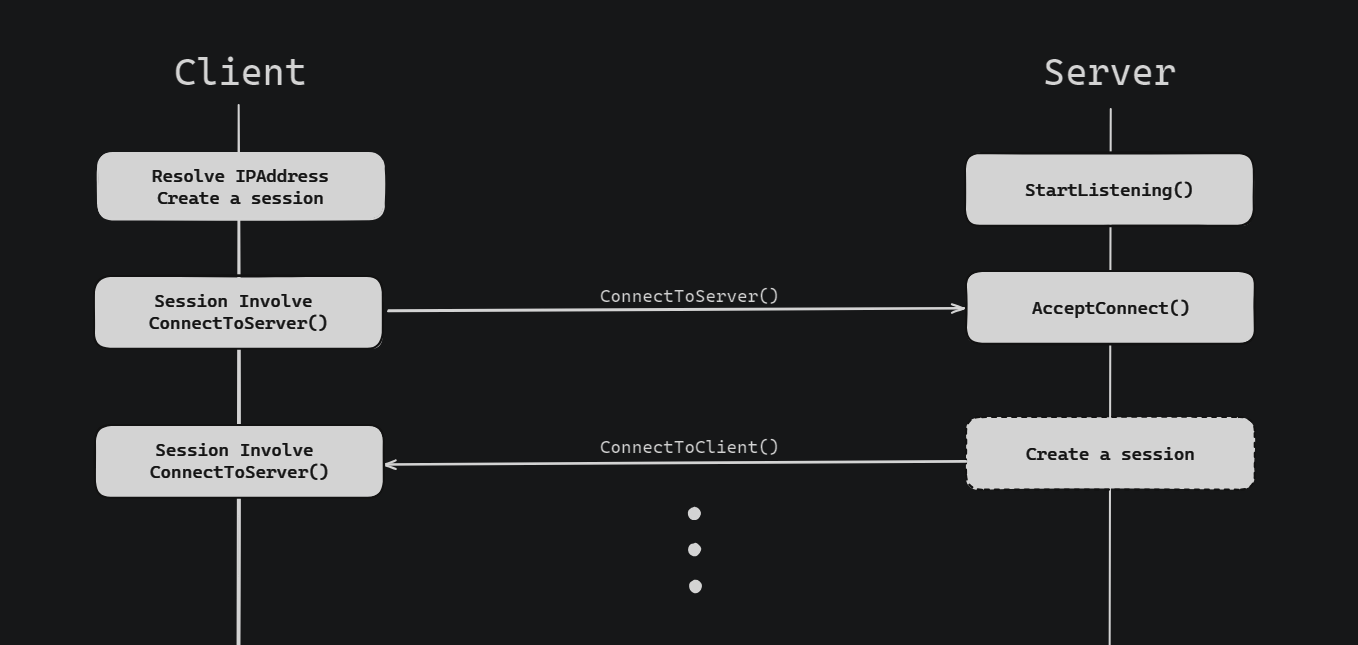
\includegraphics[width=\linewidth]{latex/architechture/connecting}
	\caption{Establish connection}
	\label{fig:handshake}
\end{figure}

\textbf{b. Nhận và gởi: }
Sơ đồ \ref{fig:network} cũng đã mô tả quá trình giao tiếp giữa các thành phần trong mạng với nhau. 
\begin{itemize}
	\item Ở quá trình \textbf{gởi}: Sau khi message được tạo bởi \textit{Client} hoặc \textit{Server}, message sẽ được kiểm tra đưa vào đúng \textit{Session} cần gởi. Message khi vào \textit{Session} sẽ được đưa vào \textit{OutcommingQueue} để chờ các gói message phía trước nó được gởi. Khi đến lượt, message sẽ được gởi thông qua hai giai đoạn: \textit{WriteHeader()} gởi Header và \textit{WriteBody()} gởi Body bằng \textit{Socket}. Việc này sẽ làm giảm sức ép lên băng thông và vẫn đảm bảo nhận đủ dữ liệu khi mà kích thước của Header là cố định còn kích thước Body đã được lưu trữ ở Header.
	\item Ở quá trình \textbf{Nhận}: Khi nhận, \textit{socket} của \textit{Session} bên nhận sẽ là nơi xử lý đầu tiên, lặp lại đúng như thứ tự gởi ở bên gởi. \textit{ReadHeader()} và \textit{ReadBody()}. Khi quá trình nhận hoàn thành, message mới sẽ được tạo và sẽ được đẩy vào \textit{IncommingQueue} để \textit{Client} hoặc \textit{Server} để xử lý.
\end{itemize}

\subsection{Thiết kế Protocol: }

Tại phần này, chúng tôi sẽ trình bày chi tiết giao thức mà Client và Server dùng để giao tiếp với nhau. 

\subsubsection{Thiết lập kết nối, cập nhật và ngắt kết nối}

\begin{itemize}
	\item \textbf{Kết nối: } Sau khi \textbf{Client} được khởi tạo và yêu cầu kết nối với \textbf{Server} đang \textit{Listening}, nếu yêu cầu được chấp nhận, \textbf{Server} sẽ phản hồi bằng cách gửi một \textit{message} có kiểu header là \textbf{SERVER\_ACCEPT}. \textbf{Client} nhận được phản hồi này và tiến hành xử lý các bước khởi tạo, hoàn tất việc thiết lập kết nối giữa hai bên.
	\item \textbf{Cập nhật: } Trong quá trình kết nối, cả hai đều liên tục trao đổi thông tin. Về phía \textbf{Server}, nó sẽ gửi các thông tin cập nhật đến màn hình Remote của \textbf{Client}, mỗi thông tin này đều được gửi dưới các \textit{message} có kiểu header là \textbf{SERVER\_UPDATE}. Về phía \textbf{Client}, có nhiều loại \textit{message} khác nhau được sử dụng để cập nhật thông tin cho \textbf{Server}. Chúng sẽ được mô tả chi tiết trong các phần tiếp theo của \textbf{Kiến trúc Protocol}.
	\item \textbf{Ngắt kết nối}Khi \textbf{Server} chủ động ngắt kết nối, nó sẽ gửi thông báo cho \textbf{Client} qua \textit{message} có kiểu header là \textbf{SERVER\_DISCONNECT}, nội dung rỗng. Tương tự, nếu \textbf{Client} chủ động ngắt kết nối, nó cũng sẽ gửi thông báo cho \textbf{Server} qua \textit{message} có kiểu header là \textbf{CLIENT\_DISCONNECT}.
\end{itemize}
	
\subsubsection{MetaData}

Giao tiếp này giúp người dùng bên \textbf{Client} và \textbf{Server} nhận được các thông tin cơ bản của nhau.

Khi \textbf{Client} được tạo, nó sẽ ngay lập tức gọi hàm để gửi các thông tin như \textit{địa chỉ IP, địa chỉ MAC},... cho \textbf{Server}, với \textit{message header} là \textbf{MetaData}.

Về phía \textbf{Server}, nó cũng sẽ gửi các thông tin cơ bản. Các thông tin này được gửi đi cùng với \textit{message} có  \textit{header} là \textbf{SERVER\_ACCEPT} đã được trình bày ở trên.

\subsubsection {Các sự kiện chuột, bàn phím}

Nội dung được trình bày sau đây là các loại \textit{message} chứa sự kiện chuột, bàn phím mà \textbf{Client} gửi tới \textbf{Server}.

Để thông tin được trình bày một cách rõ ràng và khái quát nhất, sau đây tôi sẽ liệt kê từng loại \textit{message header}, miêu tả thành phần nội dung được lưu trữ của \underline{tin nhắn mang header đó} và \underline{công việc của loại tin nhắn} đó.

\begin{itemize}
	\item \textbf{MouseClick}:  Dùng để gửi sự kiện chuột được nhấn. Chứa toạ độ tung, hoành nơi mà \textbf{Client} ấn chuột và loại nút chuột được nhấn \textit{(left, right, middle, aux1...)}.
	\item \textbf{MouseUnClick}: Dùng để gửi sự kiện chuột được nhả ra. Cũng chứa toạ độ và loại nút chuột được nhả.
	\item \textbf{DoubleClick}: Dùng để gửi sự kiện double-click được nhấn. Tương tự, chứa toạ độ và loại nút.
	\item \textbf{MouseMove}: Dùng để cập nhật vị trí con trỏ chuột. Loại tin nhắn này chỉ chứa toạ độ của chuột.
	\item \textbf{MouseWheel}: Dùng để cập nhật con lăn chuột. Chứa toạ độ và một giá trị chỉ hướng lăn của chuột.
	\item \textbf{KeyPress}: Dùng để gửi sự kiện phím được nhấn. Chỉ chứa một giá trị, đó là mã của phím.
	\item \textbf{KeyRelease}: Dùng để gửi sự kiện phím được nhả. Tương tự, chứa mã của phím.
\end{itemize}

\subsection{Capture màn hình}

Để phục vụ cho chức năng \textit{Chụp màn hình Server}, hai loại \textit{message header} \textbf{CaptureRequest} và \textbf{CaptureSend} được sử dụng.

Trong đó, khi \textbf{Client} thực thi sự kiện yêu cầu ảnh chụp màn hình từ \textbf{Server}, nó sẽ gửi một \textit{message} dưới \textit{header} \textbf{CaptureRequest}. Khi gửi lại hình cho đối phương, \textbf{Server} sẽ sử dụng \textit{header} \textbf{CaptureSend}  và nội dung của tin nhắn sẽ là mảng \textit{bit} của hình được chụp.




\subsection{Kiến trúc ứng dụng: }

Ngoài kiến trúc Network đã xây dựng, chúng tôi còn xây dựng thêm các thành phần khác cho ứng dụng nhầm hỗ trợ thêm nhiều tính năng khác:

\subsubsection{Model: }
\textit{Model} là nơi định nghĩa các đối tượng user và các thuộc tính, thao tác trên đối tượng đó. Ở đây, chúng tôi định nghĩa hai loại \textit{Model} đó là: \textit{Admin} và \textit{User}. \\
Mỗi loại \textit{Model} sẽ quy định cách thức hoạt động cho cả ứng dụng sau này khi mà \textit{Admin} có chức năng điều khiển, còn \textit{User} là người dùng được điều khiển bởi \textit{Admin}. \\
Chúng tôi đã thiết kế một vài công cụ cho \textit{Model} nhằm chức năng đăng nhập, xác thực người dùng, phân quyền người dùng, và quãn lý các User cho \textit{Admin},...


\subsubsection{User Interface: }
Thiết kế giao diện căn bản cho người dùng bằng cách phân chia thành nhiều window khác nhau như: \textbf{LoginWindow}, \textbf{MainWindow}, \textbf{CaptureWindow},...

\subsection{Nhận xét: }

\textbf{Ưu điểm: }
\begin{itemize}
	\item \textbf{Phân chia rõ ràng và độc lập}: Kiến trúc được phân chia thành các thành phần như Message, ThreadSafe Queue, Session, IClient và IServer, Giao tiếp giữa các thành phần, giúp chúng hoạt động một cách độc lập và giảm sự phụ thuộc lẫn nhau. Điều này tạo điều kiện thuận lợi cho việc phát triển, giảm thời gian kiểm tra lỗi và sửa lỗi.
	\item \textbf{Quản lý bộ nhớ và trạng thái tự động}: Session được thiết kế để quản lý bộ nhớ và trạng thái một cách tự động, giúp giảm độ phức tạp trong việc xử lý gửi nhận trong quá trình giao tiếp.
	\item \textbf{Hàng đợi ThreadSafe:} Sử dụng ThreadSafe Queue cho mọi hàng đợi tạo ra trong phần Network, giúp đảm bảo an toàn khi truy cập từ nhiều luồng thực thi khác nhau.
	\item \textbf{Quá trình phát triển: } Giúp việc phát triển dễ dàng và nhanh chóng hơn, giảm thời giam kiểm lỗi và sửa lỗi. Việc giảm thiểu sự phụ thuộc giữa các thành phần giúp dễ dàng mở rộng ứng dụng và thêm nhiều tính năng hơn khi quá trình sửa chữa và thay thế trên ít file hơn.
\end{itemize}

\textbf{Khuyết điểm: }
\begin{itemize}
	\item \textbf{Hạn chế do giới hạn kết nối}: Hiện tại, chúng tôi chỉ thiết kế duy nhất hai \textit{Session} cho mỗi Client và Server. Điều này có thể khiến cho vài tính năng khó có thể được hiện thực hóa hơn. 
	\item \textbf{Giới hạn về tốc độ}: Việc sử dụng Session chung với giao thức TCP có thể làm chậm hơn quá trình gởi nhận ảnh khi yêu cầu của người dùng là real-time. Chúng tôi đã từng xem xét đến việc sử dụng UDP cho ứng dụng. Tuy nhiên, ứng dụng được sử dụng cho người dùng trong mạng LAN nên tốc độ truyền ảnh đã nằm ở mức chấp nhận được. Ngoài ra, chúng tôi nhận thấy rằng việc truyền dữ liệu đáng tin cậy mang nhiều ưu điểm hơn trong ứng dụng Remote Desktop như bảo mật, kiểm soát luồng, đảm bảo hiệu ứng xử lý hình ảnh,...
	\item \textbf{Quá trình phát triển: } Việc phân chia thành nhiều thành phần làm cho giai đoạn đầu sẽ khá phức tạp và nặng nề. Cả với những ai muốn phát triển và đóng góp cho đồ án cũng sẽ khó tiếp cận hơn. Nhưng về sau, việc phát triển sẽ dễ dàng hơn trước nhiều.
\end{itemize}




\subsection{Thiết kế Protocol: }

Tại phần này, chúng tôi sẽ trình bày chi tiết giao thức mà Client và Server dùng để giao tiếp với nhau. 

\subsubsection{Thiết lập kết nối, cập nhật và ngắt kết nối}

\begin{itemize}
	\item \textbf{Kết nối: } Sau khi \textbf{Client} được khởi tạo và yêu cầu kết nối với \textbf{Server} đang \textit{Listening}, nếu yêu cầu được chấp nhận, \textbf{Server} sẽ phản hồi bằng cách gửi một \textit{message} có kiểu header là \textbf{SERVER\_ACCEPT}. \textbf{Client} nhận được phản hồi này và tiến hành xử lý các bước khởi tạo, hoàn tất việc thiết lập kết nối giữa hai bên.
	\item \textbf{Cập nhật: } Trong quá trình kết nối, cả hai đều liên tục trao đổi thông tin. Về phía \textbf{Server}, nó sẽ gửi các thông tin cập nhật đến màn hình Remote của \textbf{Client}, mỗi thông tin này đều được gửi dưới các \textit{message} có kiểu header là \textbf{SERVER\_UPDATE}. Về phía \textbf{Client}, có nhiều loại \textit{message} khác nhau được sử dụng để cập nhật thông tin cho \textbf{Server}. Chúng sẽ được mô tả chi tiết trong các phần tiếp theo của \textbf{Kiến trúc Protocol}.
	\item \textbf{Ngắt kết nối}Khi \textbf{Server} chủ động ngắt kết nối, nó sẽ gửi thông báo cho \textbf{Client} qua \textit{message} có kiểu header là \textbf{SERVER\_DISCONNECT}, nội dung rỗng. Tương tự, nếu \textbf{Client} chủ động ngắt kết nối, nó cũng sẽ gửi thông báo cho \textbf{Server} qua \textit{message} có kiểu header là \textbf{CLIENT\_DISCONNECT}.
\end{itemize}
	
\subsubsection{MetaData}

Giao tiếp này giúp người dùng bên \textbf{Client} và \textbf{Server} nhận được các thông tin cơ bản của nhau.

Khi \textbf{Client} được tạo, nó sẽ ngay lập tức gọi hàm để gửi các thông tin như \textit{địa chỉ IP, địa chỉ MAC},... cho \textbf{Server}, với \textit{message header} là \textbf{MetaData}.

Về phía \textbf{Server}, nó cũng sẽ gửi các thông tin cơ bản. Các thông tin này được gửi đi cùng với \textit{message} có  \textit{header} là \textbf{SERVER\_ACCEPT} đã được trình bày ở trên.

\subsubsection {Các sự kiện chuột, bàn phím}

Nội dung được trình bày sau đây là các loại \textit{message} chứa sự kiện chuột, bàn phím mà \textbf{Client} gửi tới \textbf{Server}.

Để thông tin được trình bày một cách rõ ràng và khái quát nhất, sau đây tôi sẽ liệt kê từng loại \textit{message header}, miêu tả thành phần nội dung được lưu trữ của \underline{tin nhắn mang header đó} và \underline{công việc của loại tin nhắn} đó.

\begin{itemize}
	\item \textbf{MouseClick}:  Dùng để gửi sự kiện chuột được nhấn. Chứa toạ độ tung, hoành nơi mà \textbf{Client} ấn chuột và loại nút chuột được nhấn \textit{(left, right, middle, aux1...)}.
	\item \textbf{MouseUnClick}: Dùng để gửi sự kiện chuột được nhả ra. Cũng chứa toạ độ và loại nút chuột được nhả.
	\item \textbf{DoubleClick}: Dùng để gửi sự kiện double-click được nhấn. Tương tự, chứa toạ độ và loại nút.
	\item \textbf{MouseMove}: Dùng để cập nhật vị trí con trỏ chuột. Loại tin nhắn này chỉ chứa toạ độ của chuột.
	\item \textbf{MouseWheel}: Dùng để cập nhật con lăn chuột. Chứa toạ độ và một giá trị chỉ hướng lăn của chuột.
	\item \textbf{KeyPress}: Dùng để gửi sự kiện phím được nhấn. Chỉ chứa một giá trị, đó là mã của phím.
	\item \textbf{KeyRelease}: Dùng để gửi sự kiện phím được nhả. Tương tự, chứa mã của phím.
\end{itemize}

\subsection{Capture màn hình}

Để phục vụ cho chức năng \textit{Chụp màn hình Server}, hai loại \textit{message header} \textbf{CaptureRequest} và \textbf{CaptureSend} được sử dụng.

Trong đó, khi \textbf{Client} thực thi sự kiện yêu cầu ảnh chụp màn hình từ \textbf{Server}, nó sẽ gửi một \textit{message} dưới \textit{header} \textbf{CaptureRequest}. Khi gửi lại hình cho đối phương, \textbf{Server} sẽ sử dụng \textit{header} \textbf{CaptureSend}  và nội dung của tin nhắn sẽ là mảng \textit{bit} của hình được chụp.



\input{latex/architechture/application}
\section{Gửi và nhận email}
\subsection{Nhận mail}
\begin{itemize}
\item Giao thức sử dụng: POP3.
\item Nhà cung cấp mail: Microsoft Outlook.
\item Sử dụng đa luồng để tối ưu hóa tác vụ.
\end{itemize}
Các hàm sử dụng cho quá trình nhận mail (POP3$\_$service.py):
\begin{lstlisting}
def get_mails():
\end{lstlisting}
Chức năng: Lấy toàn bộ mail đang có trong mail box, tách lấy \textit{email người gửi}, \textit{tiêu đề} và \textit{nội dung} (nếu có), đưa vào hàng đợi để luồng khác xử lý, sau đó thì xóa mail để đảm bảo không trùng lắp với thư cũ.\\
Quá trình thực hiện:
\begin{itemize}
 \item Tạo kết nối POP3 tới server (có sử dụng SSL).
 \item Gửi username (mail) và password để xác thực.
 \item Lấy số lượng mail hiện có qua lệnh \lstinline{LIST}.
 \item Lấy thông tin từng thư qua lệnh \lstinline{RETR}.
 \item Tách lấy thông tin.
 \item Xóa thư với lệnh \lstinline{DELE}.
 \item Gửi lệnh \lstinline{QUIT} ngắt kết nối.
\end{itemize} 

\begin{lstlisting}
def loop():
\end{lstlisting}
Chức năng: Do tính chất của POP3 không cập nhật thư mới, cần phải reload lại sau một khoảng thời gian, nên hàm này sẽ thực hiện việc lấy thư liên tục (gọi tới hàm \lstinline{get_mails()}) khi chương trình khởi chạy.

\subsection{Gửi mail}
\begin{itemize}
\item Giao thức sử dụng: SMTP.
\item Nhà cung cấp mail: Microsoft Outlook.
\item Sử dụng đa luồng để tối ưu hóa tác vụ.
\end{itemize}
Các hàm sử dụng cho quá trình gửi mail (SMTP$\_$service.py):
\begin{lstlisting}
def send(to_: str, subject_: str, content_, file_name):
\end{lstlisting}
Chức năng: Gửi thư đến địa chỉ \lstinline{to_}, với tiêu đề \lstinline{subject_}, nội dung \lstinline{content_} và tên file \lstinline{file_name} nếu nội dung cần gửi là file (file ảnh, video...)\\
Tham số: 
\begin{itemize}
\item \lstinline{ to_}: kiểu \lstinline{str}, là địa chỉ mail người nhận (ví dụ \lstinline{abc@gmail.com}).
\item \lstinline{subject_}: kiểu \lstinline{str}, là tiêu đề của mail.
\item \lstinline{content_}: kiểu \lstinline{str} hoặc \lstinline{bytes}. Nếu là \lstinline{str}, thực hiện gửi như văn bản bình thường. Nếu là  \lstinline{bytes}, gửi như một file với tên file là \lstinline{file_name}.
\item \lstinline{file_name}: kiểu \lstinline{str}, tên file (mặc định là "x.txt").
\end{itemize}
Quá trình thực hiện:
\begin{itemize}
\item Tạo kết nối SMTP tới server (có sử dụng TLS) .
\item Gửi username (mail) và password để xác thực.
\item Soạn thư với định dạng \href{https://datatracker.ietf.org/doc/html/rfc1341}{MIME multipart}.
\item Nếu thư kiểu text, attach \lstinline{MIME text}.
\item Nếu thư kiểu bytes, attach \lstinline{MIME application} với tên file.
\item Gửi payload đến server và đóng kết nối.
\end{itemize}

\begin{lstlisting}
def safe_send(to_:str, subject_:str, content_, file_name):
\end{lstlisting}
Chức năng: Là wrapper cho hàm \lstinline{send}, thực hiện xử lý ngoại lệ: thực hiện gửi thư lại cho đến khi thành công (do trong một số trường hợp, gửi mail quá nhanh server sẽ từ chối nên phải thực hiện lại).\\
Tham số: tương tự \lstinline{send}.

\begin{lstlisting}
def send_threading(to_:str, subject_:str, content_, file_name = "x.txt"):
\end{lstlisting}
Chức năng: tạo threading để gửi thư, các tham số sẽ truyền trực tiếp vào cho hàm \lstinline{safe_send}. (Đây là hàm sẽ được gọi để gửi thư khi được import)\\

\section{Các hàm xử lý yêu cầu}
\subsection{Phân tích câu lệnh}
Hàm phân tích câu lệnh được định nghĩa là:
\begin{lstlisting}
def command_parser(message, sender_email_address):
\end{lstlisting}
Chức năng: phân tích câu lệnh được gửi đến, gọi hàm tương ứng với yêu cầu của câu lệnh.\\
Tham số:
\begin{itemize}
\item \lstinline{message}: câu lệnh được gửi đến
\item \lstinline{sender_email_address}: địa chỉ email của người gửi.
\end{itemize}
Không có giá trị trả về.\\

Hàm \lstinline{get_corresponding_ip}
\begin{lstlisting}
def get_corresponding_ip(sender_email_address):
\end{lstlisting}
Chưc năng: lấy ra địa chỉ IP tương ứng với \lstinline{sender_email_address}.\\
Tham số:
\begin{itemize}
\item \lstinline{sender_email_address}: địa chỉ email của người gửi.
\end{itemize}
Trả về địa chỉ IP tương ứng, trả về None nếu không tồn tại.
\subsection{Module mail$\_$handler}
Các hàm được định nghĩa trong module handle.py được sử dụng để xử lý các yêu cầu từ người dùng.
\begin{lstlisting}
def authorize(email, ip):
\end{lstlisting}
Chức năng: authorize địa chỉ email với IP tương ứng.\\
Thám số: 
\begin{itemize}
\item \lstinline{email}: địa chỉ email.
\item \lstinline{ip}: kiểu tuple(str, int) chứa địa chỉ ip và port của client gửi tới.
\end{itemize}
Trả về True nếu thành công, False nếu không thành công.

\begin{lstlisting}
def list_ip():
\end{lstlisting}
Chức năng: trả về danh sách các địa chỉ IP đang được kết nối.

\begin{lstlisting}
def disconnect(email):
\end{lstlisting}
Chức năng: disconnect địa chỉ email hiện tại với IP tương ứng.
Tham số:
\begin{itemize}
\item \lstinline{email}: địa chỉ IP tương ứng.
\end{itemize}
Không có giá trị trả về.

\begin{lstlisting}
def find_corresponding_email(ip_address):
\end{lstlisting}
Chức năng: tìm địa chỉ email tương ứng với IP được truyền vào.
Tham số:
\begin{itemize}
\item \lstinline{ip_address}: kiểu tuple(str, int) chứa địa chỉ ip và port của client gửi tới.
\end{itemize}
Trả về: địa chỉ email tương ứng đang điều khiển địa chỉ IP này.

\begin{lstlisting}
def delete_ip_from_list(ip_address):
\end{lstlisting}
Chức năng: xóa địa chỉ IP ra khỏi danh sách IP kết nối.
Tham số: 
\begin{itemize}
\item \lstinline{ip_address}: kiểu tuple(str, int) chứa địa chỉ ip và port của client gửi tới.
\end{itemize}
Không có giá trị trả về.

\begin{lstlisting}
def remove_this_connection(conn, ip_address):
\end{lstlisting}
Chức năng: loại bỏ kết nối tương ứng với IP.
Tham số:
\begin{itemize}
\item \lstinline{conn}: socket tương ứng.
\item \lstinline{ip_address}: kiểu tuple(str, int) chứa địa chỉ ip và port của client gửi tới.
\end{itemize}
Không có giá trị trả về.

\begin{lstlisting}
def __init__():
\end{lstlisting}
Chức năng: khởi tạo những giá trị liên quan.
\subsection{Process/Application}
Server sẽ gửi lệnh \textbf{APP$\_$PRO} đến client, sau đó sẽ gửi số tương ứng với lệnh.
\begin{itemize}
\item Gửi số 1 nếu ta cần đưa ra danh sách process/application. Sau đó gửi message là \textbf{APPLICATION} hoặc \textbf{PROCESS} tương ứng với yêu cầu của lệnh đến client. Client nhận thông điệp rồi gửi lại danh sách application/process dưới dạng một data frame.
\item Gửi số 0 nếu ta cần kill một process/application. Sau đó ta sẽ gửi ID/PID của đối tượng cần kill. Client nhận thông điệp rồi gửi thông tin về quá trình kill lại cho server.
\end{itemize}
Các hàm cho quá trình này như sau:\\
\begin{itemize}
\item Ở server (mail$\_$handler.py, app$\_$process$\_$server.py):
\begin{lstlisting}
def list_process(ip_address):
\end{lstlisting}
Chức năng: gửi yêu cầu đến client, nhận kết quả rồi gửi mail lại cho người dùng.\\
Tham số: 
\begin{itemize}
\item \lstinline{ip_address}: kiểu tuple(str, int) chứa địa chỉ ip và port của client gửi tới.
\end{itemize}
Trả về: Không có giá trị trả về.
\begin{lstlisting}
def _list(conn:socket.socket, s):
\end{lstlisting}
Chức năng: gửi yêu cầu danh sách tiến trình/ứng dụng đến client, nhận kết quả từ client.\\
Tham số: 
\begin{itemize}
\item \lstinline{conn}: socket kết nối server với client.
\item \lstinline{s}: chuỗi, có giá trị là \textbf{PROCESS} hoặc \textbf{APPLICATION}, thể hiện yêu cầu gửi danh sách tiến trình hoặc ứng dụng.
\end{itemize}
Trả về: Danh sách tiến trình/ứng dụng ở dạng chuỗi.
\begin{lstlisting}

def send_kill(conn:socket.socket, process_id): 
\end{lstlisting}
Chức năng: gửi yêu cầu tắt một tiến trình.\\
Tham số: 
\begin{itemize}
\item \lstinline{conn}: socket kết nối server với client.
\item \lstinline{process_id}: id của tiến trình cần tắt.
\end{itemize}
Trả về: kết quả kill thành công/không thành công.\\
Thư viện sử dụng: pickle, struct, pandas.
\item Ở client (app$\_$process$\_$client.py):
\begin{lstlisting}
def app_process(client):
\end{lstlisting}
Chức năng: nhận yêu cầu từ server, xử lý yêu cầu rồi gửi lại kết quả tương ứng. \\
Tham số: 
\begin{itemize}
\item \lstinline{client}: socket kết nối server với client.
\end{itemize}
Trả về: Không có giá trị trả về.\\
Thư viện sử dụng: pickle, psutil, struct, os, subprocess.\\
Bên cạnh đó, server còn có các hàm (được cung cấp sẵn) phụ trách việc nhận dữ liệu:
\begin{lstlisting}
def recvall(sock, size):
def receive(client):
\end{lstlisting}
Ngoài ra, client còn có các hàm (được cung cấp sẵn) phục vụ việc gửi dữ liệu cho server và xử lý các yêu cầu về application/process trên máy.
\begin{lstlisting}
def send_data(client, data):
def list_apps():
def list_processes():
def kill(pid):
\end{lstlisting}
\end{itemize}






\subsection{Chụp màn hình}
Server sẽ gửi lệnh \textbf{LIVESCREEN} đến client, sau đó sẽ gửi lệnh tương ứng với thời gian cần chụp màn hình, thời gian mặc định là $0.5$ giây. Thời gian chụp không nên quá nhiều, vì giới hạn dung lượng tệp đính kèm trong email. Sau đó, server sẽ nhận ảnh gửi từ client, tạo thành một video.\\
Các hàm cho quá trình này như sau:
\begin{itemize}
\item Ở server (mail$\_$handler.py):
\begin{lstlisting}
def capture_screen(ip_address, time=0.5):
\end{lstlisting}
Chức năng: gửi yêu cầu chụp màn hình đến cho client, nhận hình ảnh từ client gửi lại, tạo video, gửi mail trả lời cho người dùng.\\
Tham số: 
\begin{itemize}
\item \lstinline{ip_address}: kiểu tuple(str, int) chứa địa chỉ ip và port của client gửi tới.
\item \lstinline{time}: thời gian chụp màn hình (giây).
\end{itemize}
Không có giá trị trả về. 
\item Ở client:
\begin{lstlisting}
def capture_screen(client):
\end{lstlisting}
Chức năng: nhận yêu cầu chụp màn hình từ server, chụp màn hình liên tục rồi gửi từng ảnh lại cho server.\\
Tham số: 
\begin{itemize}
\item \lstinline{client}: socket kết nối server với client.
\end{itemize}
Không có giá trị trả về.\\
Thư viện sử dụng: ImageGrab, io, time.\\
Ngoài ra, ở server còn có hàm sau dùng để tạo video từ những ảnh chụp màn hình nhận được từ client, sử dụng thư viện os, cv2.
\begin{lstlisting}
def create_video(image_folder: str):
\end{lstlisting}

\end{itemize}



\subsection{Webcam}
Server sẽ gửi lệnh \textbf{WEBCAM} đến client, sau đó sẽ gửi lệnh tương ứng với thời gian cần chụp màn hình, thời gian mặc định là $5$ giây. Client nhận thông điệp từ server, quay màn hình webcam trong khoảng thời gian đó, rồi gửi lại video cho server.\\
Các hàm cho quá trình này như sau:
\begin{itemize}
\item Ở server (mail$\_$handler.py):
\begin{lstlisting}
def capture_webcam(ip_address, time=5):
\end{lstlisting}
Chức năng: gửi yêu cầu ghi lại webcam đến cho client, nhận video từ client gửi về, gửi mail trả lời cho người dùng.\\
Tham số: 
\begin{itemize}
\item \lstinline{ip_address}: kiểu tuple(str, int) chứa địa chỉ ip và port của client gửi tới.
\item \lstinline{time}: thời gian ghi hình webcam (giây).
\end{itemize}
Không có giá trị trả về.
\item Ở client (webcam$\_$client.py):
\begin{lstlisting}
def run(conn: socket.socket):
\end{lstlisting}
Chức năng: nhận yêu cầu từ server, quay màn hình webcam, gửi lại file video cho server.\\
Tham số: 
\begin{itemize}
\item \lstinline{conn}: socket kết nối server với client.
\end{itemize}
Không có giá trị trả về.\\
Thư viện sử dụng: tempfile, cv2, time.\\
Ngoài ra, ở client còn có hàm sau dùng để gửi file về cho server:
\begin{lstlisting}
def send_file(conn: socket.socket):
\end{lstlisting}
\end{itemize}




\subsection{Keylogger}
Server sẽ gửi lệnh \textbf{KEYLOG} cho client. Do thiết kế của các hàm có sẵn cho việc keylog ở client, server sẽ gửi 2 lệnh \textbf{HOOK} đến client để lấy các hành động giữa 2 lần. Sau đó, một lệnh \textbf{PRINT} được gửi đến client để client gửi dữ liệu về các phím nhấn đã bắt được cho server. Server nhận kết quả từ client.\\
Các hàm cho quá trình này như sau:
\begin{itemize}
\item Ở server ((mail$\_$handler.py): 
\begin{lstlisting}
def keylog(ip_address, time=10):
\end{lstlisting}
Chức năng: gửi yêu cầu keylog đến client, nhận kết quả từ client gửi về, gửi mail trả lời cho người dùng.\\
Tham số: 
\begin{itemize}
\item \lstinline{ip_address}: kiểu tuple(str, int) chứa địa chỉ ip và port của client gửi tới.
\item \lstinline{time}: thời gian keylog (giây).
\end{itemize}
Không có giá trị trả về.\\
Sử dụng hàm \lstinline{sleep} của thư viện time.
\item Ở client (keylogger$\_$client.py):
\begin{lstlisting}
def keylog(client):
\end{lstlisting}
Chức năng: nhận lệnh từ server, bắt các phím nhấn rồi gửi kết quả lại cho server, ngoài ra còn có chức năng phụ để có thể khóa phím người dùng (Không được đề cập trong chương trình).\\
Tham số: 
\begin{itemize}
\item \lstinline{client}: socket kết nối server với client.
\end{itemize}
Không có giá trị trả về.\\
Thư viện sử dụng: threading, keyboard, pynput.keyboard.\\
Ngoài ra, ở client còn có các hàm để bổ trợ cho hàm \lstinline{keylog} trong việc bắt phím nhấn cũng như gửi kết quả lại cho server.

\begin{lstlisting}
def keylogger(key):
\end{lstlisting}
Chức năng: Dựa vào \lstinline{global} flag (nhận giá trị 0, 1, 2, 4), thực hiện xử lý \lstinline{key} lấy được từ \lstinline{Listener} trong hàm \lstinline{listen()} như sau:\\
+ Thay thế \lstinline{space} thành ký tự khoảng trắng\\
+ Thay thế phím ' thành chuỗi phù hợp \\
+ Lọc bỏ toàn bộ ký tự ' dư thừa \\
+ Nối vào câu \\
Tham số: 
\begin{itemize}
\item \lstinline{key}: Phím được bắt từ quá trình Listener
\end{itemize}
Không có giá trị trả về.\\

\begin{lstlisting}
def _print(client):
\end{lstlisting}
Chức năng: Gửi câu đang được ghi về server\\
Tham số: 
\begin{itemize}
\item \lstinline{client}: socket kết nối server với client..
\end{itemize}
Không có giá trị trả về.

\begin{lstlisting}
def listen():
\end{lstlisting}
Chức năng: Tạo thread mới để ghi bàn phím (sử dụng hàm keylogger để xử lý)\\
Không có giá trị trả về.\\

\end{itemize}
\subsection{Registry}
Sẽ có 2 loại lệnh được gửi cho client:
\begin{itemize}
\item Liệt kê subkey: SERVER sẽ gửi lệnh \textbf{REGISTRY} cùng với \textbf{LIST} và đường dẫn (ví dụ như là HKEY$\_$CURRENT$\_$USER, HKEY$\_$CURRENT$\_$USER/System), client sẽ trả về danh sách các subkey tương ứng.
\item Cập nhật key: SERVER sẽ gửi lệnh \textbf{REGISTRY} cùng với \textbf{UPDATE} và đường dẫn tới key, giá trị mới của key, và kiểu dữ liệu (kiểu dữ liệu thường thuộc 1 trong 4 loại: REG$\_$BINARY, REG$\_$DWORD, REG$\_$QWORD, REG$\_$SZ).
\end{itemize}

Các hàm cho quá trình này như sau:
\begin{itemize}
\item Ở server (mail$\_$handler.py):\\
\begin{lstlisting}
def registry_list(ip_address, full_path):
\end{lstlisting}
Chức năng: gửi các câu lệnh để liệt kê subkey với đường dẫn là \lstinline{full_path} đến client, sau đó nhận về danh sách subkey, gửi mail trả lời cho người dùng.\\
Tham số: 
\begin{itemize}
\item \lstinline{ip_address}: kiểu tuple(str, int) chứa địa chỉ ip và port của client gửi tới.
\item \lstinline{full_path}: kiểu str, là đường dẫn cần liệt kê subkey.
\end{itemize}
Không có giá trị trả về.

\begin{lstlisting}
def registry_update(ip_address, absolute_path, value, data_type):
\end{lstlisting}
Chức năng: gửi câu lệnh để cập nhật giá trị entry tới client, nhận về kết quả, gửi mail trả lời người dùng.\\
Tham số: 
\begin{itemize}
\item \lstinline{ip_address}: kiểu tuple(str, int) chứa địa chỉ ip và port của client gửi tới.
\item \lstinline{absolute_path}: đường dẫn tới entry cần cập nhật giá trị.
\item \lstinline{value}: giá trị mới cho entry, giá trị này KHÔNG được có khoảng trắng.
\item \lstinline{data_type}: kiểu dữ liệu của entry cần cập nhật.
\end{itemize}
Không có giá trị trả về.


\item Ở client (registry$\_$client.py):
\begin{lstlisting}
def registry_handle(conn):
\end{lstlisting}
Chức năng: xử lý các yêu cầu gửi đến rồi trả kết quả lại cho server.\\
Tham số: 
\begin{itemize}
\item \lstinline{conn}: socket kết nối server với client.
\end{itemize}
Trả về: 

\begin{lstlisting}
def identify_hkey(value_list):
\end{lstlisting}
Chức năng: Xác định hive từ đường dẫn đã được tách\\
Tham số: 
\begin{itemize}
\item \lstinline{ip_address}: kiểu tuple(str, int) chứa địa chỉ ip và port của client gửi tới.
\item \lstinline{full_path}: kiểu str, là đường dẫn cần liệt kê subkey.
\end{itemize}
Trả về: giá trị hive tương ứng.

\begin{lstlisting}
def get_value_of_key(key):
\end{lstlisting}
Chức năng: lấy giá trị của \lstinline{key}.\\
Tham số: 
\begin{itemize}
\item \lstinline{key}: key cần lấy giá trị.
\end{itemize}
Trả về: giá trị tại \lstinline{key}.

\begin{lstlisting}
def get_sub_keys(key):
\end{lstlisting}
Chức năng: lấy ra các subkeys của \lstinline{key}.\\
Tham số: 
\begin{itemize}
\item \lstinline{key}: key cần lấy các subkeys.
\end{itemize}
Trả về: subkeys của \lstinline{key}.

\begin{lstlisting}
def list_all_registry_entries(registry_path, reg_dict):
\end{lstlisting}
Chức năng: liệt kê danh sách các entries trong 1 đường dẫn registry.\\
Tham số: 
\begin{itemize}
\item \lstinline{registry_path}: đường dẫn registry cần liệt kê.
\item \lstinline{reg_dict}: dictionary dùng để lưu kết quả.
\end{itemize}
Không có giá trị trả về.\\
Ngoài ra, client có các hàm được cung cấp sẵn để giúp cho quá trình xử lý yêu cầu trên registry.
\begin{lstlisting}
def parse_data(full_path):
def dec_value(c):
def str_to_bin(s):
def str_to_dec(s):
def set_value(full_path, value, value_type):
\end{lstlisting}

\end{itemize}


\subsection{Directory}
Sẽ có 2 loại lệnh được gửi cho client:
\begin{itemize}
\item Liệt kê files/directories: SERVER sẽ gửi lệnh \textbf{DIR} cùng với \textbf{LIST} và đường dẫn (ví dụ như là C:/Users/admin), client sẽ trả về danh sách các files/directories trong đường dẫn tương ứng.
\item Cập nhật key: SERVER sẽ gửi lệnh \textbf{DIR} cùng với \textbf{COPY}, đường dẫn tới file cần copy cũng như thư mục mà file sẽ được copy vào.
\end{itemize}
\textbf{Lưu ý:} các đường dẫn KHÔNG được có khoảng trắng.\\
Các hàm cho quá trình này như sau :
\begin{itemize}
\item Ở server (mail$\_$handler.py):
\begin{lstlisting}
def dir_list(ip_address, path_to_folder):
\end{lstlisting}
Chức năng: gửi yêu cầu liệt kê danh sách files/directories đến client, nhận kết quả, gửi mail trả lời người dùng.\\
Tham số: 
\begin{itemize}
\item \lstinline{ip_address}: kiểu tuple(str, int) chứa địa chỉ ip và port của client gửi tới.
\item \lstinline{path_to_folder}: đường dẫn cần liệt kê. 
\end{itemize}
Không có giá trị trả về.

\begin{lstlisting}
def dir_copy(ip_address, src_path, dst_path):
\end{lstlisting}
Chức năng: gửi yêu cầu copy file đến client, nhận kết quả, gửi mail trả lời người dùng.\\
Tham số: 
\begin{itemize}
\item \lstinline{ip_address}: kiểu tuple(str, int) chứa địa chỉ ip và port của client gửi tới.
\item \lstinline{src_path}: đường dẫn tới file cần copy.
\item \lstinline{dst_path}: thư mục mà file sẽ được copy vào.
\end{itemize}
Không có giá trị trả về.

\item Ở client (directory$\_$tree$\_$client.py):
\begin{lstlisting}
def directory_handle(conn):
\end{lstlisting}
Chức năng: xử lý các yêu cầu về liệt kê/copy từ server, gửi kết quả lại cho server.\\
Tham số: 
\begin{itemize}
\item \lstinline{conn}: socket kết nối server với client.
\end{itemize}
Không có giá trị trả về.
\end{itemize}



\subsection{Shutdown/log out/restart}
Server sẽ gửi lệnh \textbf{SHUTDOWN} hoặc \textbf{LOGOUT} hoặc \textbf{RESTART}, tùy theo yêu cầu, đến client. Client nhận lệnh rồi thực hiện. Khi client thực hiện nhóm lệnh này, kết nối của client tương ứng với server sẽ bị ngắt, đồng thời email đang điều khiển client này cũng bị disconnect, nếu muốn kết nối lại thì phải authorize lại.\\
Các hàm cho quá trình này như sau:
\begin{itemize}
\item Ở server:\\
mail$\_$handler.py:
\begin{lstlisting}
def shut_down(ip_address):
def logout(ip_address):
def restart(ip_address):
\end{lstlisting}
Chức năng: gọi hàm gửi yêu cầu đến client, gửi mail xác nhận cho người dùng.\\
Tham số: 
\begin{itemize}
\item \lstinline{ip_address}: kiểu tuple(str, int) chứa địa chỉ ip và port của client gửi tới.
\end{itemize}
Không có giá trị trả về.

shutdown$\_$logout$\_$server.py:
\begin{lstlisting}
def shutdown(conn):
def logout(conn):
def restart(conn):
\end{lstlisting}
Chức năng: gửi yêu cầu tương ứng đến client.\\
Tham số: 
\begin{itemize}
\item \lstinline{conn}: socket kết nối server với client.
\end{itemize}
Không có giá trị trả về.
\item Ở client (shutdown$\_$logout$\_$client.py):
\begin{lstlisting}
def shutdown_logout(conn, msg):
\end{lstlisting}
Chức năng: xử lý yêu cầu shutdown/log out/restart từ server.\\
Tham số: 
\begin{itemize}
\item \lstinline{conn}: socket kết nối server với client.
\item \lstinline{msg}: thông điệp gửi từ server.
\end{itemize}
Không có giá trị trả về. 
\end{itemize}




% nhiều quá :( hjx :((
\section{Demo}
Video demo của chương trình được đăng tải tại \href{https://youtu.be/aqded2HKIt0}{đây}.
\newpage
\setcounter{secnumdepth}{0}
\section{Lời cảm ơn}
%\addcontentsline{toc}{section}{Lời cảm ơn}
Trong quá trình thực hiện đồ án này, những kiến thức về Mạng máy tính được giảng dạy bởi thầy Đỗ Hoàng Cường đã giúp ích chúng em rất nhiều trong việc giải quyết các vấn đề. Ngoài ra, source code TelePC từ thầy đã giúp nhóm có thể dễ dàng hơn khi xử lý các yêu cầu của đồ án. Nhóm chúng em xin cảm ơn thầy vì những kiến thức cũng như những chia sẻ này ạ.\\
Bên cạnh đó, những kỹ năng lập trình socket được các giáo viên hướng dẫn thực hành là thầy Lê Hà Minh và thầy Nguyễn Thanh Quân truyền đạt đã góp phần không nhỏ trong việc hoàn thành đồ án này.\\
Ngoài ra, nhóm cũng xin chân thành cảm ơn những người bạn đã đóng góp ý kiến, góp phần hoàn thiện đồ án.
\begin{flushright}
Thành phố Hồ Chí Minh, tháng 6 năm 2022
\end{flushright}


\end{document}